%%%%%%%%%%%%%%%%%%%%%%%%%%%%%%%%%%%%%%%%%
% Beamer Presentation
% LaTeX Template
% Version 1.0 (10/11/12)
%
% This template has been downloaded from:
% http://www.LaTeXTemplates.com
%
% License:
% CC BY-NC-SA 3.0 (http://creativecommons.org/licenses/by-nc-sa/3.0/)
%
%%%%%%%%%%%%%%%%%%%%%%%%%%%%%%%%%%%%%%%%%

%----------------------------------------------------------------------------------------
%	PACKAGES AND THEMES
%----------------------------------------------------------------------------------------
  
\documentclass[aspectratio=169]{beamer}
\usetheme[progressbar=frametitle]{metropolis}
\usepackage{appendixnumberbeamer}

\usepackage[backend=biber, citestyle=authoryear, bibencoding=utf8]{biblatex}
\addbibresource{./bibs/digital-ads.bib}
\addbibresource{./bibs/adaptive-design.bib}
 
\mode<presentation> {

% The Beamer class comes with a number of default slide themes
% which change the colors and layouts of slides. Below this is a list
% of all the themes, uncomment each in turn to see what they look like.

%\usetheme{default}
%\usetheme{AnnArbor}
%\usetheme{Antibes}
%\usetheme{Bergen}
%\usetheme{Berkeley}
%\usetheme{Berlin}
% \usetheme{Boadilla} %
%\usetheme{CambridgeUS} %
%\usetheme{Copenhagen}
%\usetheme{Darmstadt}
%\usetheme{Dresden}
%\usetheme{Frankfurt}
%\usetheme{Goettingen}
%\usetheme{Hannover}
%\usetheme{Ilmenau}
%\usetheme{JuanLesPins}
%\usetheme{Luebeck}
%\usetheme{Madrid} %
%\usetheme{Malmoe}
%\usetheme{Marburg}
%\usetheme{Montpellier}
%\usetheme{PaloAlto}
%\usetheme{Pittsburgh}
%\usetheme{Rochester}
%\usetheme{Singapore} %
%\usetheme{Szeged}
%\usetheme{Warsaw}

% As well as themes, the Beamer class has a number of color themes
% for any slide theme. Uncomment each of these in turn to see how it
% changes the colors of your current slide theme.

%\usecolortheme{albatross}
%\usecolortheme{beaver} %
%\usecolortheme{beetle}
%\usecolortheme{crane}
%\usecolortheme{dolphin}
%\usecolortheme{dove}
%\usecolortheme{fly}
%\usecolortheme{lily}
%\usecolortheme{orchid}
%\usecolortheme{rose}
%\usecolortheme{seagull}
%\usecolortheme{seahorse}
%\usecolortheme{whale}
%\usecolortheme{wolverine}

%\setbeamertemplate{footline} % To remove the footer line in all slides uncomment this line
%\setbeamertemplate{footline}[page number] % To replace the footer line in all slides with a simple slide count uncomment this line

\setbeamertemplate{navigation symbols}{} % To remove the navigation symbols from the bottom of all slides uncomment this line
}

\usepackage{graphicx} % Allows including images
\usepackage{booktabs} % Allows the use of \toprule, \midrule and \bottomrule in tables

\usepackage{accents}
\newcommand{\ubar}[1]{\underaccent{\bar}{#1}}
\usepackage{stmaryrd}


\usepackage{pgfplots}
\pgfplotsset{width=7cm,compat=1.9}

\usepackage{tabularx}
\newcolumntype{Y}{>{\centering\arraybackslash}X}\newcolumntype{Y}{>{\centering\arraybackslash}X}
	\newcommand\fnote[1]{\captionsetup{font=footnotesize}\caption*{#1}}
	\newcolumntype{K}[1]{>{\centering\arraybackslash}p{#1}}
\newcolumntype{P}[1]{>{\centering\arraybackslash}p{#1}}

\usepackage{amssymb}
\usepackage{amsmath}
\usepackage{algorithm}
\usepackage{algpseudocode}

% Add significance note with \starnote
\newcommand{\starnote}{\figtext{* p $<$ 0.1, ** p $<$ 0.05, *** p $<$ 0.01. Standard errors in parentheses.}}

\usepackage{siunitx} % centering in tables
\sisetup{
detect-mode,
tight-spacing		= true,
group-digits		= false ,
input-signs		= ,
input-symbols		= ( ) [ ] - + *,
input-open-uncertainty	= ,
input-close-uncertainty	= ,
table-align-text-post	= false
        }
\makeatother



\DeclareMathOperator*{\argmin}{argmin}

%----------------------------------------------------------------------------------------
%	TITLE PAGE
%----------------------------------------------------------------------------------------

\title[title]{Applied Economics PhD Report 2023} % The short title appears at the bottom of every slide, the full title is only on the title page

% Authors
\author[Nandan Rao]{Nandan Rao}

\author[me]{Nandan Rao\\[3mm]Advisor: Caterina Calsamiglia\\Tutor: Francesc Trillas} 


\date[\today] {\today} % Date, can be changed to a custom date

\begin{document}

\begin{frame}
\titlepage
\end{frame}


%----------------------------------------------------------------------------------------
%	PRESENTATION SLIDES
%----------------------------------------------------------------------------------------

%------------------------------------------------
\section{Research Purpose and Scope}


\begin{frame}
\frametitle{Developing Online Research Methodologies} 

Randomized control trials can be used to measure the impact of population-level policies and interventions. 

By construction, randomized control trials often involve recruiting and gathering data from willing study participants, some of whom will be treated by the intervention. 

Online and digital interventions are affordable to scale up quickly. Offline recruitment and data gathering, however, is both expensive and suffers from an external validity problem when attempting to transfer those results to online populations. 

\end{frame}


\begin{frame}
\frametitle{Developing Online Research Methodologies} 

My research develops methodologies for performing end-to-end survey-based research entirely online.

I seek to solve two problems that currently exist for economists across multiple sub-fields: 
\begin{enumerate}
\item The need to evaluate the impact of an intervention which is performed online, such as an online ad campaign or a mobile app distributed online. 
\item The need to run surveys affordably and quickly to gather novel data, or higher-frequency data, that can only be gather through asking people questions. 
\end{enumerate}

The second need becomes highly relevant in the context of the first need, however it is more general. 

\end{frame}



\begin{frame}
\frametitle{Strategy for Applying Methodologies} 

Much of the work I present in this dissertation will be based on randomized control trials for impact evaluation, highly collaborative in nature due to their significant budgetary requirements. 

What they share, however, are methodologies for recruiting participants and gathering data from them entirely online, affordably and at scale. These methodologies form the core of my scientific contribution in this dissertation.  

The usefulness of these methodologies will not be restricted to economics, but they will be of special interest to economists whose work often relies on quantitative data and randomized control trials to measure causal impacts. 

\end{frame} 

\begin{frame}
\frametitle{Components of the dissertation} 

My dissertation will consist of three papers:

\begin{enumerate}
\item An RCT testing the impact of online ads on attitudes, knowledge, beliefs, and behaviors. 
\item An RCT testing the impact of mobile apps on attitudes, knowledge, beliefs, and behaviors. 
\item A methodology for dynamically optimizing representative survey recruitment with online advertising and results replicating important population-level social surveys.
\end{enumerate} 

\end{frame}

\begin{frame}
  \frametitle{Continuation of a Body of Work} 

My work in the final paper lays out new methodologies that the previous two papers use to perform real-world impact evaluations that would otherwise be difficult or cost-prohibitive.

Beyond the usefulness already proved, however, this also lays the grounds for future work that continues to build on the potential of dynamically optimizing recruitment, paralleling the recent advances in adaptive experimental design\footcite{Kasy2021,Atan2020}. This opens the door for surveying methodologies that maintain cost-effectiveness while improving quality beyond what is possible with contemporary methods, including the ones presented here. 

\end{frame}

\section{Can Facebook Ads Prevent Malaria?}
\begin{frame}
\frametitle{Paper 1: Can Facebook Ads Prevent Malaria?}

Status: Near complete. 

Presented: 

\begin{itemize}
\item MIT CODE (Conference on Digital Experimentation / Massachusetts Institute of Technology), November 2021.
\item QME (Quantitative Marketing and Economics / University of Chicago) Conference, September 2023. 
\end{itemize}

Is being submitted to journals in Q1 2024. 

\end{frame}

\begin{frame}
\frametitle{Paper 1: Can Facebook Ads Prevent Malaria?}

Problem: Digital ad campaigns are increasingly used for social good and public health objectives. However, effectiveness measures are limited to direct response metrics (clicks, likes) or short-term ``brand-lift'' surveys which are limited in scope\footcite{Shawky2019,atheycovid2023}. 

Ideally we would have both random assignments of ads and measures of long-term behavior disconnected from the ad itself. 
  
\end{frame}


\begin{frame}
\frametitle{Paper 1: Can Facebook Ads Prevent Malaria?}

This paper contains two randomized control trials: 

\begin{enumerate}
\item Cluster-randomized trial with repeated panel for the duration of the actual, full-scale campaign. 
\item Individually-randomized field experiment to test the impact of the ad content from the actual campaign. 
\end{enumerate}
  
\end{frame}



\begin{frame}
\frametitle{Paper 1: Can Facebook Ads Prevent Malaria?}

\begin{columns}
\column{0.5\linewidth}
\begin{figure}[]
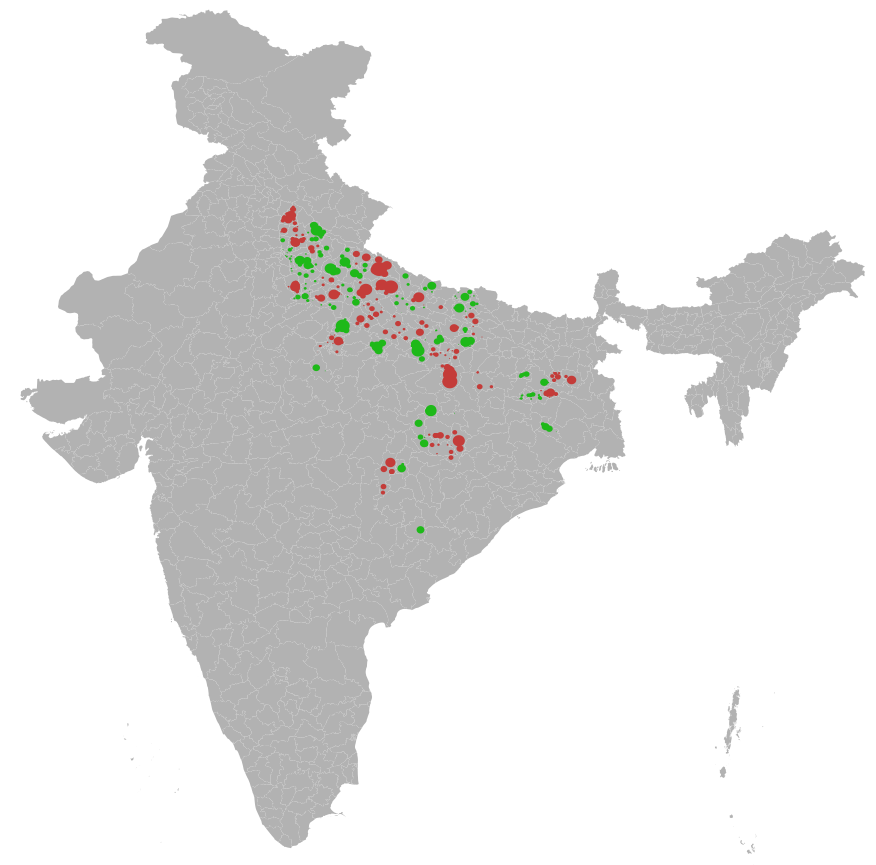
\includegraphics[width=200px]{resources/india-targeting-surveys-only.png} 
\end{figure}    
\column{0.5\linewidth}

80 districts: 40 treatment and 40 control. Used circles for Facebook targeting, fit within districts centered around populated areas. Control districts will be withheld (``punched out'') of the campaign. 
\end{columns}
\end{frame}


\begin{frame}
\frametitle{Paper 1: Can Facebook Ads Prevent Malaria?}

\begin{figure}[]
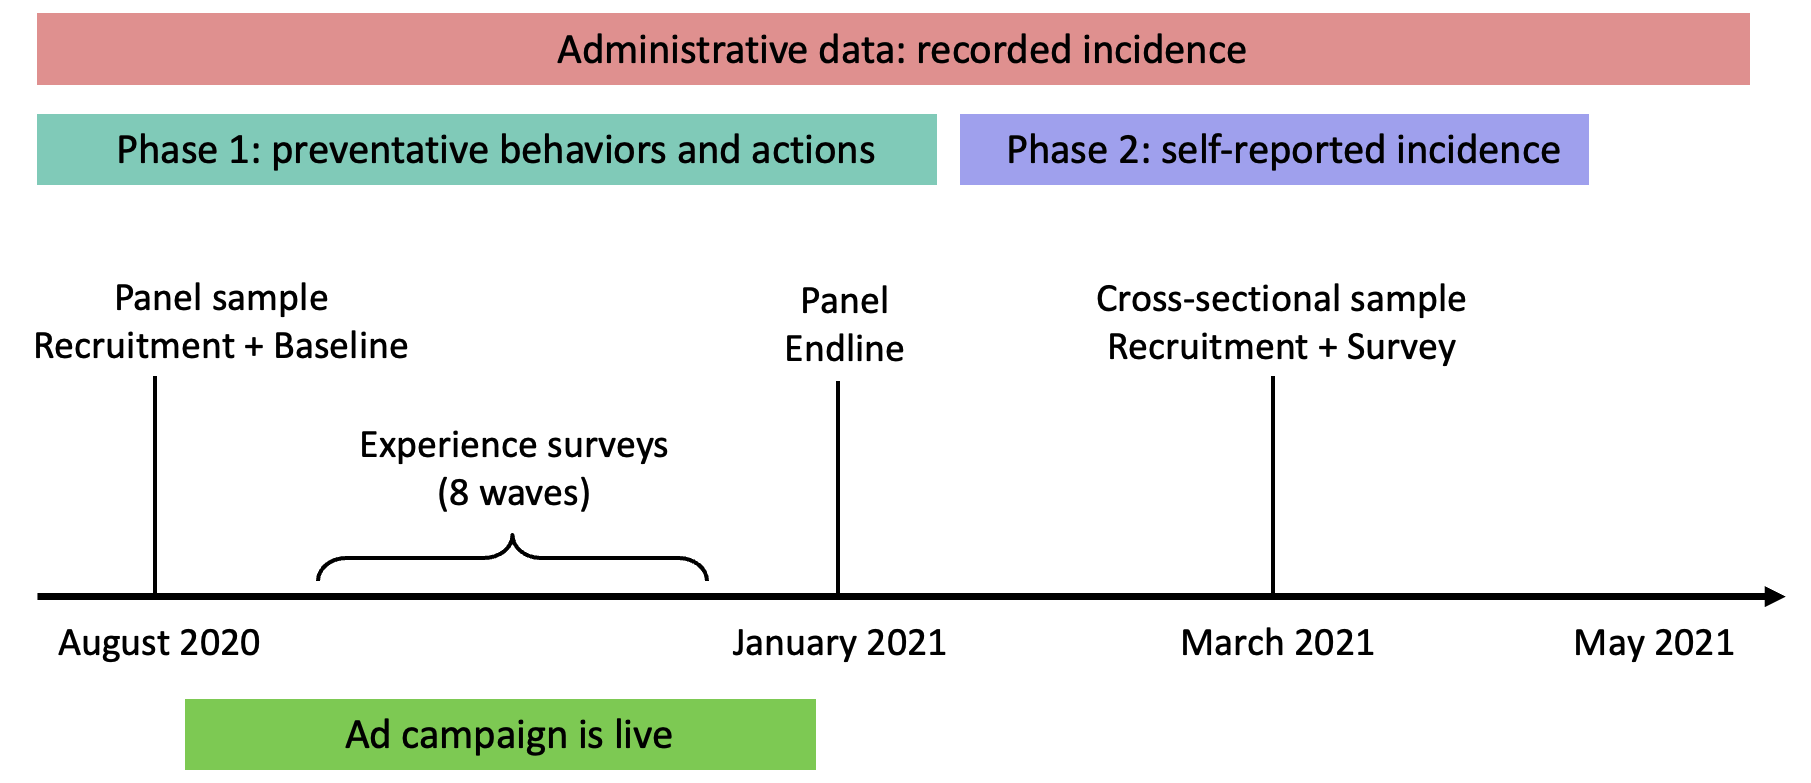
\includegraphics[width=400px]{resources/Timeline.png} 
\end{figure}    
  
\end{frame}


\begin{frame}
\frametitle{Paper 1: Can Facebook Ads Prevent Malaria?}
Problem: Those most at risk for malaria are underrepresented on social media. In particular: those living in non-solid dwellings have malaria incidence at twice the rate of those in solid dwellings.

Solution: Stratify our recruitment by dwelling-type (2), in addition to district (80), creating 160 strata. 
  
\end{frame}

\begin{frame}
\frametitle{Paper 1: Can Facebook Ads Prevent Malaria?}

By stratifying by dwelling-type, using Facebook's ``Lookalike'' audience to target the group, we increase the representivity of that otherwise underrepresented group and ensure we can measure heterogenous effects across this variable of interest: 

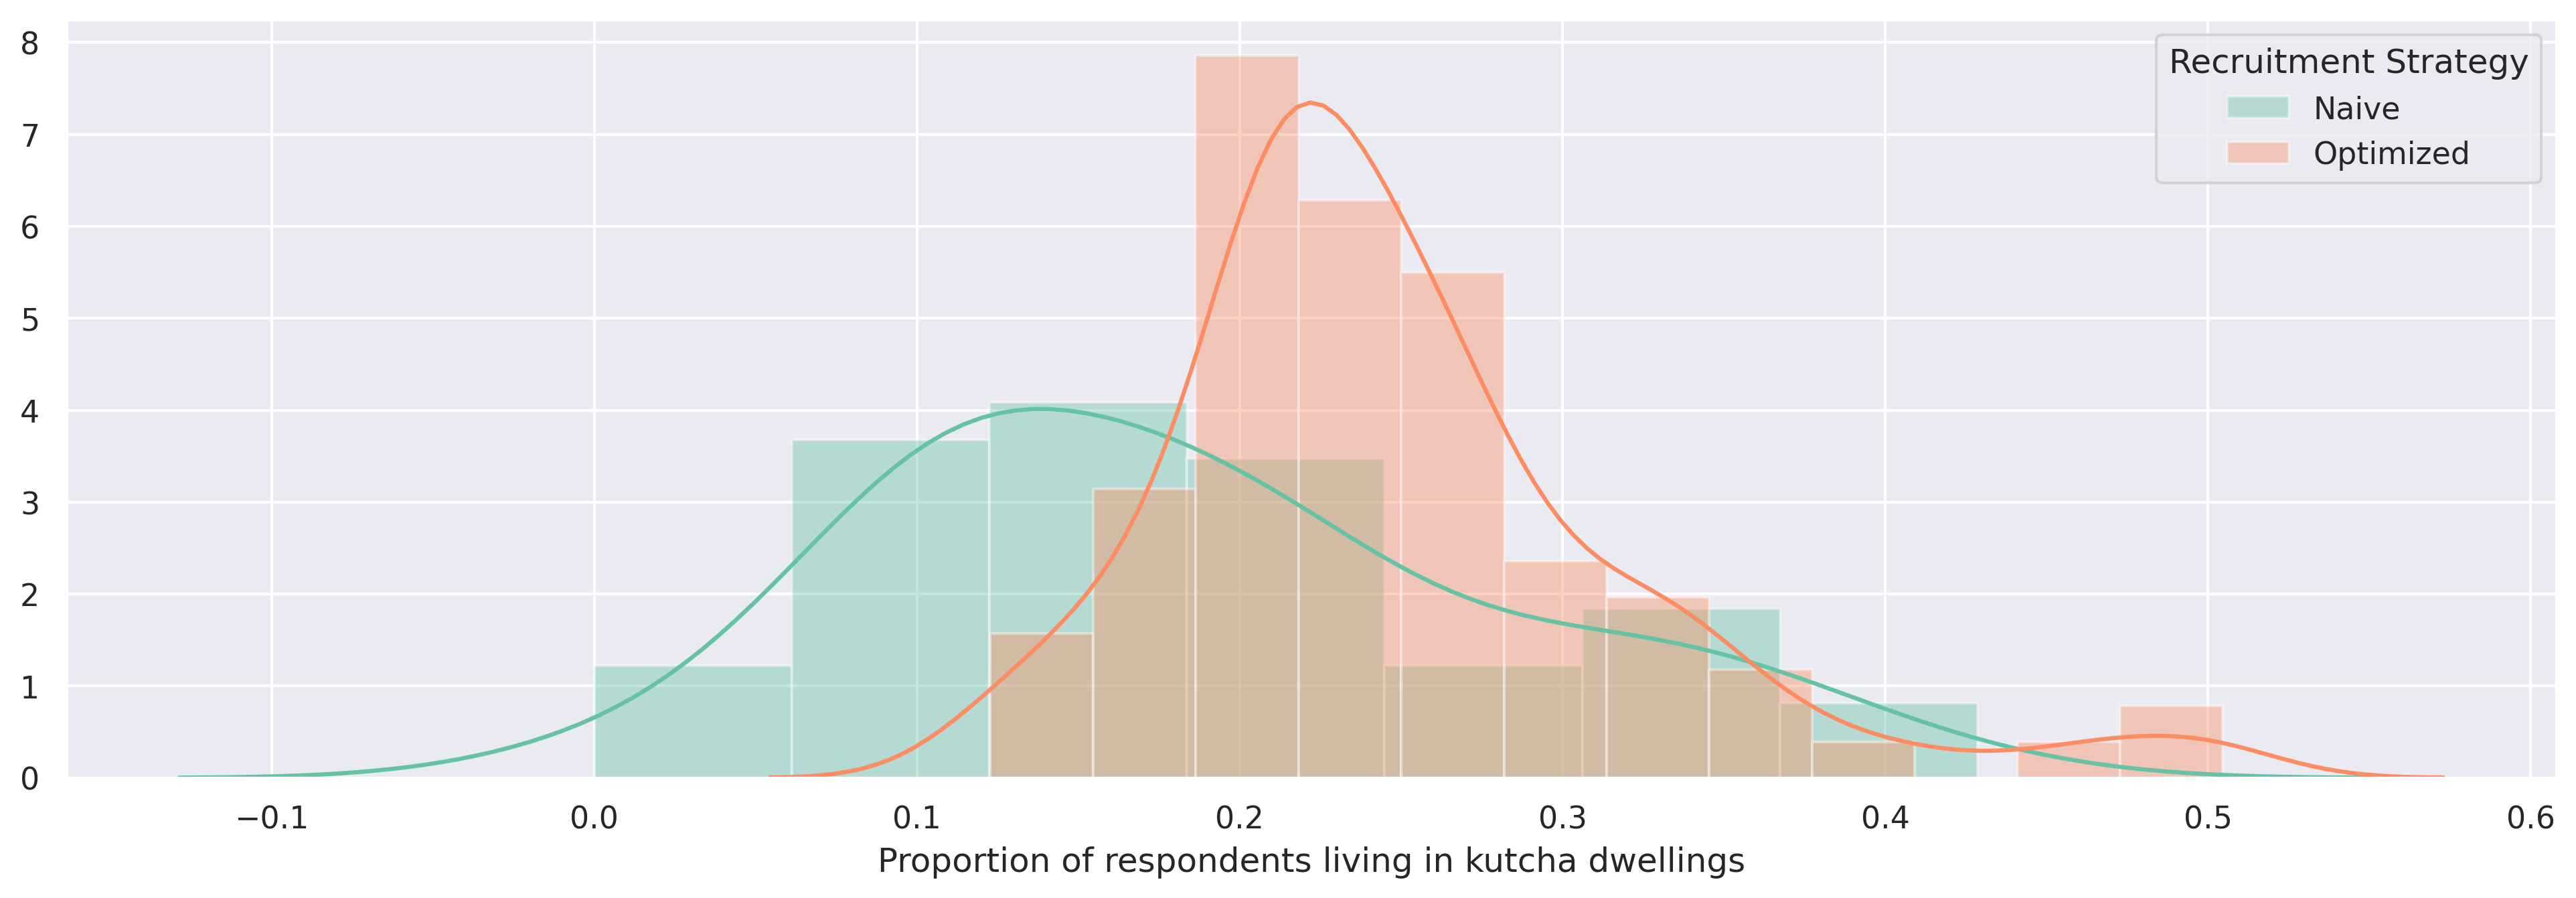
\includegraphics[width=380px]{resources/optimization-kutcha-proportion.png} 
  
\end{frame}


\begin{frame}
\frametitle{Paper 1: Can Facebook Ads Prevent Malaria?}

We look at several outcomes, but two of special interest: 

\begin{enumerate}
\item Self-reported behavior, recorded in the repeated panel survey, about whether the reporting individual slept under a mosquito net the previous night, and how many of their household members as well. 
\item Administrative data on malaria incidence, collected at district level. 
\end{enumerate}
  
\end{frame}

\begin{frame}
\frametitle{Paper 1: Can Facebook Ads Prevent Malaria?}

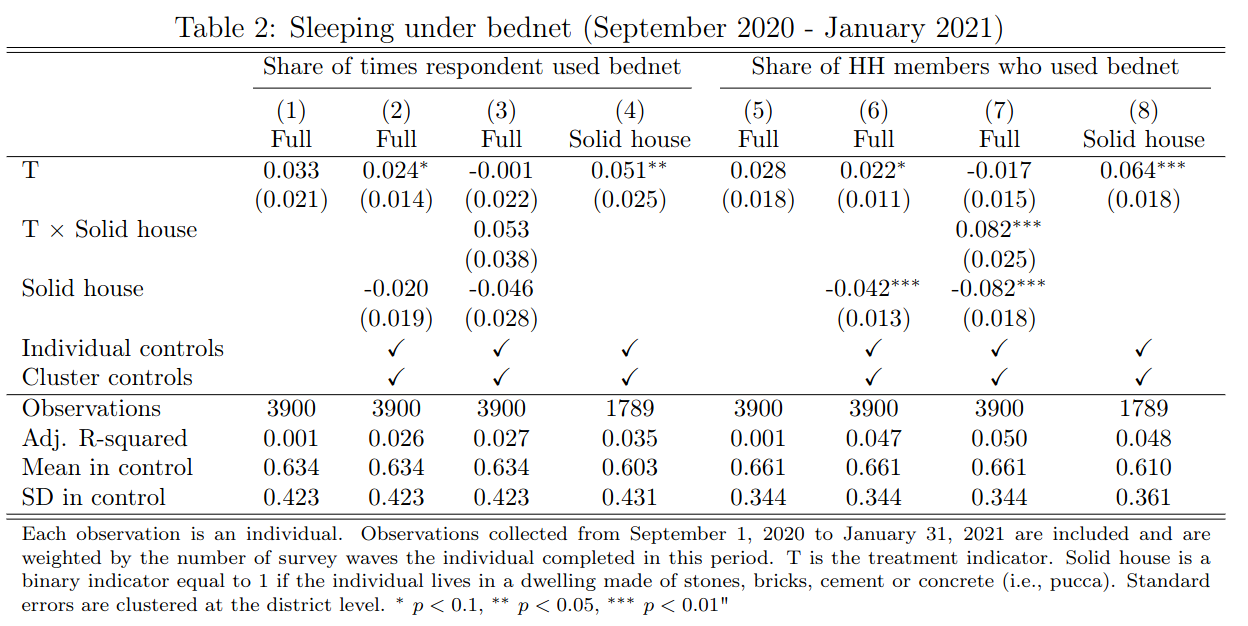
\includegraphics[width=380px]{resources/sleeping-panel-regression.png} 
  
\end{frame}



\begin{frame}
\frametitle{Paper 1: Can Facebook Ads Prevent Malaria?}

\begin{columns}
  

\column{0.7\linewidth}

\begin{figure}[]
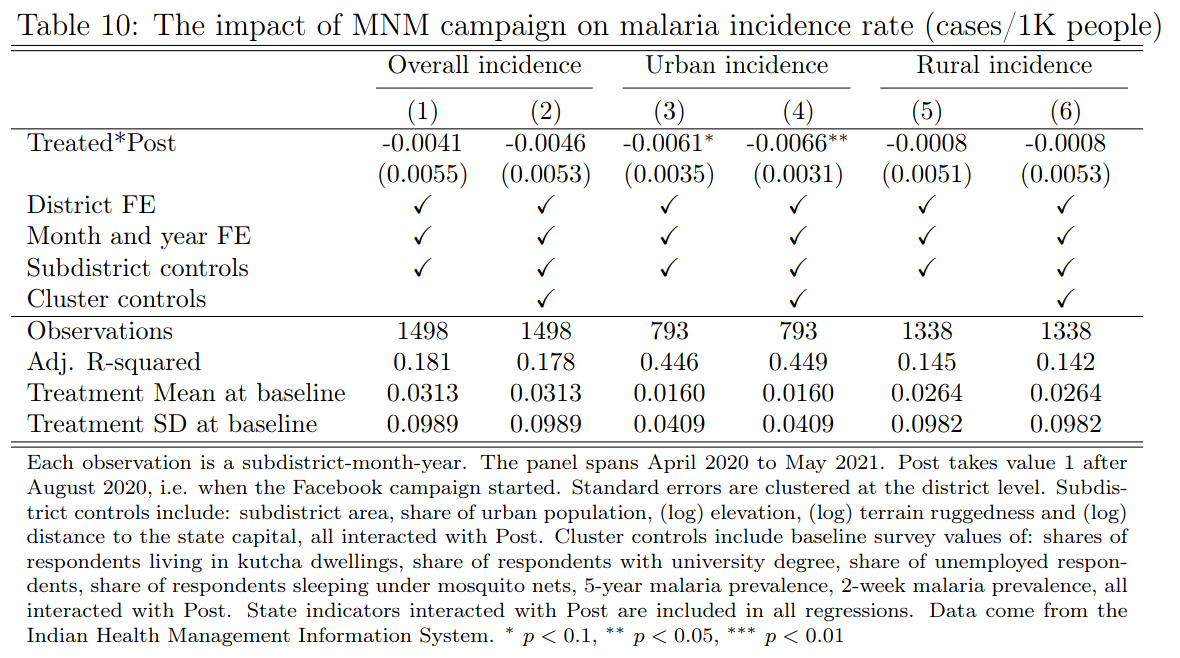
\includegraphics[width=300px]{resources/incidence-regression.png} 
\end{figure} 

\column{0.3\linewidth}

In urban areas (where 85\% of dwellings are solid), we see a decrease from 16/million to 10/ million, or about a 40\% improvement. 
   
\end{columns}
  
\end{frame}

\begin{frame}
\frametitle{Paper 1: Can Facebook Ads Prevent Malaria?}

So we know the ad campaign had an impact on those in solid dwellings and those in urban areas. The impact was significant and cost-effective (estimated at \$4.50 per case avoided). 

But why did it not impact those in non-solid dwellings? Was it the material, the targetting, or is it not possible to reach them via social media? 

To measure the effect of the material itself, we perform a second, individually-randomized experiment. 
  
\end{frame}


\begin{frame}
\frametitle{Paper 1: Can Facebook Ads Prevent Malaria?}


\begin{figure}[]
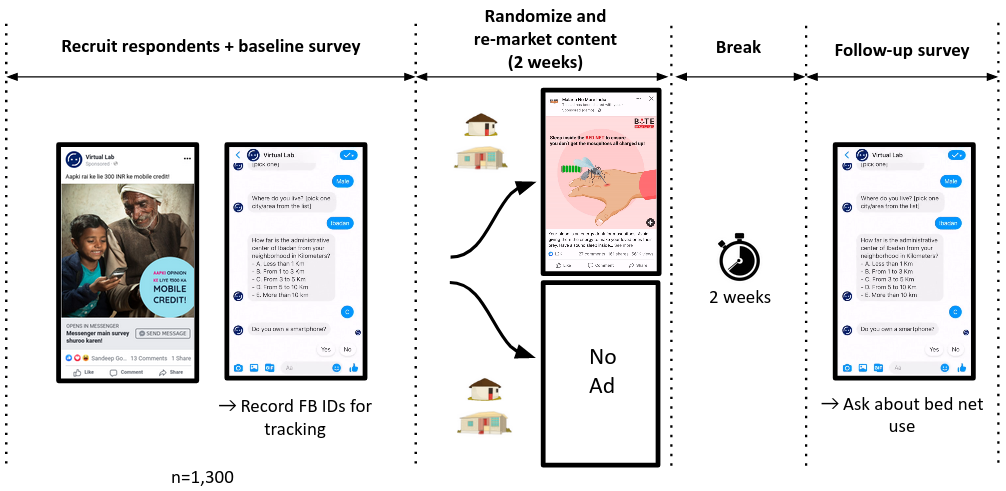
\includegraphics[width=380px]{resources/individual-study-flow.png} 
\end{figure} 

\end{frame}


\begin{frame}
\frametitle{Paper 1: Can Facebook Ads Prevent Malaria?}


\begin{columns}
  \column{0.7\linewidth}

\begin{figure}[]
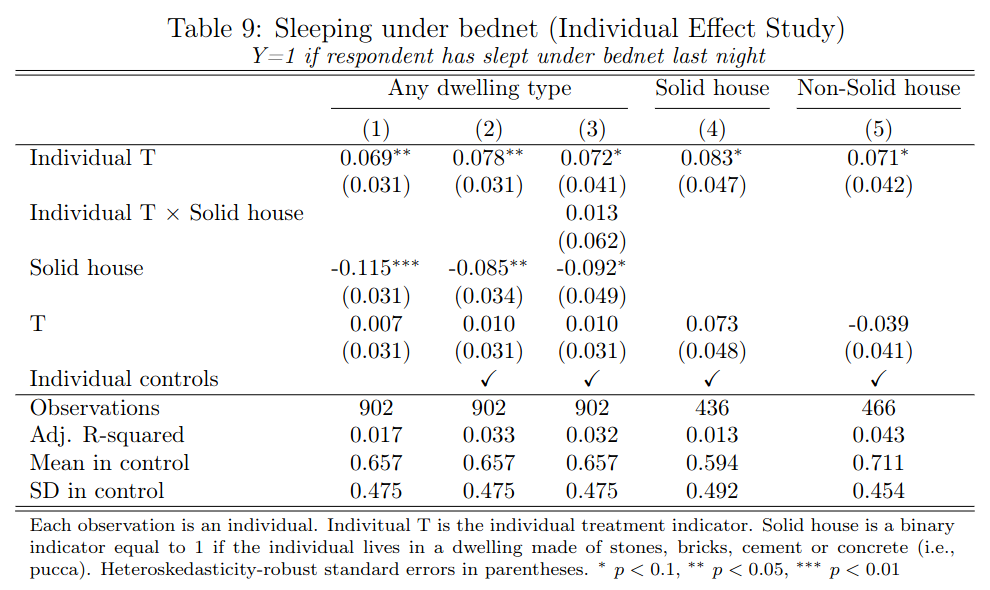
\includegraphics[width=280px]{resources/individual-effect-results.png} 
\end{figure} 

\column[10cm]{0.3\linewidth}

When we run campaigns targeted directly at individuals in a balanced sample, we find significant treatment effects across the entire population, and subgroup estimates are of similar size. 
\end{columns}

\end{frame}

\begin{frame}
  \frametitle{Paper 1: Can Facebook Ads Prevent Malaria?}

We introduce two novel methods for measuring the impact of an ad campaign: one with stratified sampling and repeated panel surveys (``experience sampling'') to measure behavior across groups. The other using remarketing techniques to test the impacts of a real ad campaign on a specific group of individuals. 

We find that this content was effective in changing behavior and that the behavior led to impacts of malaria incidence measurable from administrative data. The method was cost-effective, but did not impact the most vulnerable. However, further results show it could have impacted the most vulnerable with more sophisticated (and costly) targeting. 

\end{frame}

\section{Measuring the Impact of Apps}


\begin{frame}
\frametitle{Paper 2: Apps in Development Contexts}

Status: In Progress

Data Collection: 
\begin{enumerate}
\item First RCT finished: N=1800, Serbia/Bulgaria, initial analysis finished. Working paper submitted for review. Partner: UNICEF.
\item Second RCT in progress: N=4800, Nigeria, Senegal, Bangladesh. Third pilot under way now. Full study launches Q1 2024. Partner: The World Bank. 
\end{enumerate}

These studies will be two separate papers and the one included in my dissertation will be determined after they are finished. They have many methodological similarities. 

Estimated Finish Date: November 2024



\end{frame}

\begin{frame}
\frametitle{Paper 2: Apps in Development Contexts}

Both studies share a similar design: 

\begin{enumerate}
\item Outcomes of interest are measured both before and after treatment, via online surveys or assessments. 
\item An intent-to-treat (ITT) effect will be measured from the impact of random assignment on the difference in outcome before and after treatment (DinD). 
\item Takeup among the treated will be measured objectively with app usage data linked to recruitment surveys. 
\item Studies are subject to two-sided non-compliance, however takeup is assumed to be monotonically positive under treatment. 
\item The treatment effect on the treated (ToT) will be measured with a two-staged least squares model using random assignment as the instrumental variable.  
\end{enumerate}

\end{frame}


\begin{frame}
\frametitle{Paper 2: Apps in Development Contexts}

This leads to the following regression model for the ITT effect:

$$
y_{i} - y^{b}_i = \gamma_1 + \beta T_{i} + \gamma_2X_{i} + \epsilon_i
$$

Where $y_i$ represents the outcome of interest for individual $i$ measured after treatment, $T_i$ represents the random treatment assignment, $X_i$ a set of control variables and $y^b_i$ represents the outcome of interest measured before treatment. The parameter of interest will be the treatment effect, $\beta$. 

\end{frame}


\begin{frame}
\frametitle{Paper 2: Apps in Development Contexts}

And the following two-stage model for the ToT effect: 

\begin{align*}
y_{i} - y^{b}_i &= \gamma_1 + \beta \hat{z}_{i} + \gamma_2X_{i} + \epsilon_i \\  
z_{i} &= \gamma_3 + \gamma_4 T_{i} + \gamma_5X_{i} + \delta_i
\end{align*}  


Where $z_i$ is a binary indicator of takeup based on the recorded app-usage data and $\hat{z_i}$ the predicted takeup based on the first stage regression. Once again, parameter of interest is $\beta$

\end{frame}

\begin{frame}
\frametitle{Paper 2: Study 1: Teaching Parenting Skills}

\begin{figure}[H]

\includegraphics[width=360px]{resources/bebbo-illustration.jpg} 
\end{figure}

\end{frame}

\begin{frame}
\frametitle{Paper 2: Study 1: Teaching Parenting Skills}

Bebbo is an app for parents, developed by UNICEF. They had no rigorous way of measuring the effectiveness of the app on actually changing parenting knowledge, attitudes, and behavior. 

We designed an RCT that could be performed entirely online, in two different countries, to measure the impact the app has on parents who use it.

We developed ads run on social media to recruit study participants in Bulgaria and Serbia.
\end{frame}


\begin{frame}
\frametitle{Paper 2: Study 1: Teaching Parenting Skills}
Recruitment Ads: 

\begin{figure}
\begin{subfigure}{}

\includegraphics[width=100px]{resources/recruitment/558.png} 
\end{subfigure}
\begin{subfigure}{}

\includegraphics[width=100px]{resources/recruitment/639.png} 
\end{subfigure}
\begin{subfigure}{}

\includegraphics[width=100px]{resources/recruitment/742.png} 
\end{subfigure}

\end{figure}

\end{frame}

\begin{frame}
  \frametitle{Paper 2: Study 1: Teaching Parenting Skills}

We recruited 2616 pts in Serbia and 1689 in Bulgaria. Upon recruitment, respondents were administered the baseline survey and the treatment group was invited to download the app via the provided link. 

After approximately 4-6 weeks, we resurveyed everyone again. 1327 in Serbia and 750 in Bulgaria completed the second survey, for a retention rate of 50\% and 45\% respectively. 

\end{frame}

\begin{frame}
\frametitle{Paper 2: Study 1: Teaching Parenting Skills} 

We measure 8 distinct outcomes for the experiment, covering knowledge, attitudes, and behavior. After controlling for multiple testing, we do not find any significant impact of treatment, encouragement of downloading the app, Bebbo.

\begin{enumerate}
\item Low takeup (28\%). Potentially driven by high pre-exposure (55\% knew, 23\% had used). 
\item Relatively low usage among takeup (12\% used more than a day). 
\item Ceiling effects on some of the outcomes.
\item Survey effects on knowledge outcomes. 
\end{enumerate}

\end{frame}


\begin{frame}
\frametitle{Paper 2: Study 1: Teaching Parenting Skills} 

One of the primary outcomes of interest was the ability for the treatment to impact parenting knowledge. Unfortunately, the questions that made up the two indices in the survey instrument both suffered from quite serious ceiling effects: 
\begin{figure}[H]
\includegraphics[width=340px]{resources/plots/Original Data - Knowledge and Awareness.png}  
\end{figure}   

\end{frame}

\begin{frame}
\frametitle{Paper 2: Study 1: Teaching Parenting Skills} 


\begin{columns}
  \column{0.7\linewidth}

\begin{figure}[H]
\includegraphics[width=260px]{resources/png/pooled:-ols---endline---knowledge-and-awareness.png}  
\end{figure} 

\column{0.3\linewidth}  
Regressions do not show any significant effect on knowledge outcomes, outcomes that are most likely to be impacted by the treatment in short time. 

\end{columns}

\end{frame}

\begin{frame}
\frametitle{Paper 2: Study 1: Teaching Parenting Skills} 

To understand what is happening, it can be instructive to look at the raw pre- and post-treatment results for three groups: control, treatment without takeup, treatment with takeup. 

What we find is that all three groups improve in their scores between baseline and endline surveys, indicating a potential survey effect: respondents are asked about their knowledge about particular aspects of parenting, and if they don't know, they may go seek the knowledge. Those who download the app might seek the knowledge through the app, but those in the other groups find other means to do the same. 

\end{frame}

\begin{frame}
\frametitle{Paper 2: Study 1: Teaching Parenting Skills} 

\begin{figure}[H]
\includegraphics[width=380px]{resources/plots/pre_post/health_knw.png}  
\end{figure}   
\end{frame}
  
\begin{frame}
\frametitle{Paper 2: Study 1: Teaching Parenting Skills} 

There is some suggestive evidence that those who choose to download and use the app may be less knowledgeable, in particular regarding vaccines.

However, due to the study design, our ability to measure the impact of the app on parenting knowledge is masked by both the potential impacts of the survey itself along with strong ceiling effects. 
  
\end{frame}


\begin{frame}
\frametitle{Paper 2: Study 2: Teaching Kids to Read}

Second RCT: Mobile Apps for Early Childhood Literacy 

The purpose of this study is to measure the impact of an app for early-childhood literacy developed by the organization Curious Learning. In-field, in-person RCTs have proven effectiveness, but the question remains as to what the effect might be at scale, when delivered online. 

\end{frame}


\begin{frame}
\frametitle{Paper 2: Study 2: Teaching Kids to Read}

This is designed as a multi-country randomized control trial across three countrie: Nigeria, Senegal, and Bangladesh. 

We will recruit 1600 parents with young children in each country to participate in our study. Each parent will pick a child and administer them an online reading proficiency test. 

After the first test, the treatment group will be invited to download the reading app and encouraged to offer it to their kid. The control group, ``business as usual,'' will be encouraged to read to their children. 

\end{frame}


\begin{frame}
\frametitle{Paper 2: Study 2: Teaching Kids to Read}

Parents will be recruited by targeting them with social media ads and offering an incentive. The sample will be representative across geographic by optimizing ad spend across urban and rural geographics to ensure proper representation. 

The survey will take place in a chatbot. The chatbot is integrated with the assessment such that high scores will be excluded from the survey, and such that downloading can be tracked in the app usage data. 

Assessments will be provided at the beginning and end of a 2-week period starting from initial recruitment. 

\end{frame}

\section{Paper 3: Recruiting Survey Participants Online}
\begin{frame}

\frametitle{Paper 3: Recruiting Survey Participants Online }  

Status: In Progress

Data Collection: Starts February 2024.

Estimated Finish Date: December 2024.

Presented: 

\begin{itemize}
\item MIT CODE (Conference on Digital Experimentation / Massachusetts Institute of Technology), November 2021.
\item QME (Quantitative Marketing and Economics / University of Chicago) Conference, September 2023. 
\end{itemize}


\end{frame}

\begin{frame}
\frametitle{Paper 3: Recruiting Survey Participants Online }  

This paper shows that the process of recruiting a realistic sample to estimate a population parameter of interest with a survey questionnaire can be formulated as an optimization problem subject to budget constraints.

We show the usefulness of this formulation by recruiting a sample online using this methodology. We show that it is both significantly cheaper and faster than traditional methods. We ask our sample select questions of interest from the General Social Survey (GSS), the American Time Use Survey (ATUS), and the Current Population Survey (CPS). We compare our results to the gold standard surveys. 

\end{frame}




\begin{frame}
\frametitle{Paper 3: Recruiting Survey Participants Online }  

Problems: 

\begin{enumerate}
\item Non-response rates are rising for all survey methodologies. 
\item Random Digit Dialing was an innovation from the 60s and 70s that brought probabilistic sampling frames at a much cheaper price than previous methodologies, but non-response rates have now reached 91\%.
\item Companies build survey ``panels'' with RDD that can be used for research, however they are not cheap and not available in all places - either all countries or in specific regions. 
\end{enumerate}

\end{frame}

\begin{frame}
\frametitle{Paper 3: Recruiting Survey Participants Online }  

Opportunities:

\begin{enumerate}
\item Digital advertising can be used to micro-target ads at people all over the world, in countries and specific regions. 
\item Advances in post-stratification weighting have proven the ability to approach similar estimates and probabilistic samples with convenience samples. 
\end{enumerate}

\end{frame}


\begin{frame}
\frametitle{Motivation - weighting}

\begin{figure}[H]
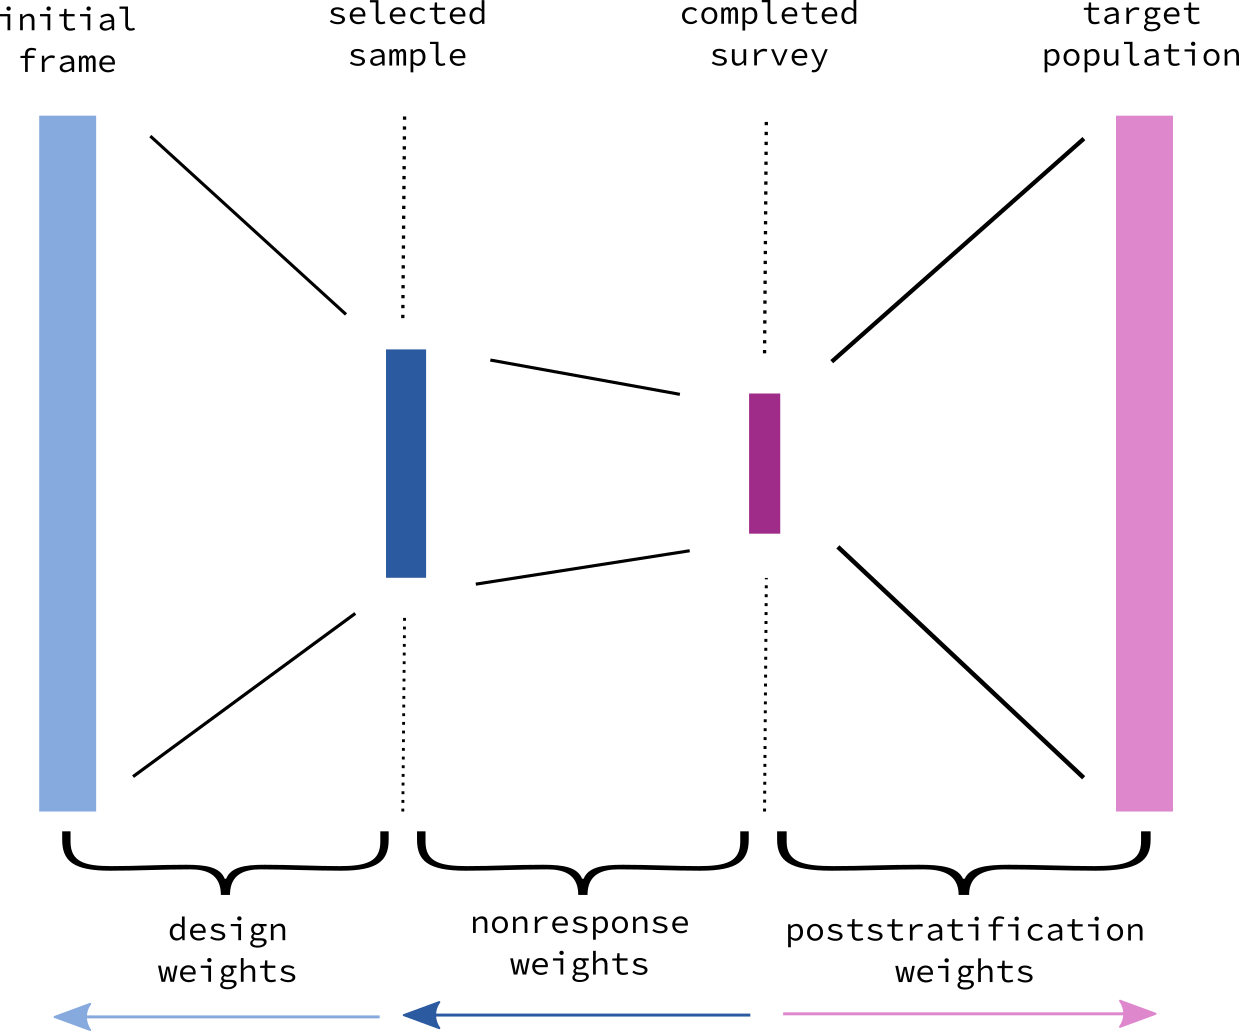
\includegraphics[height=200px]{resources/weighting.png}
\end{figure}
\end{frame}


\begin{frame}
\frametitle{Setup}

Poststratification weighting can be done in many ways, but we will consider the simplest case.

We want to estimate e a population parameter $Y$ via sampling and measurement. We will assume that the researcher wishes to use the stratified mean for a set of strata $h \in H$ (mutually exclusive cells) with an assigned weight for each stratum $W_h$, which we will denote $\bar{y}$:


$$
\hat{Y} := \sum_h W_h\bar{y}_h
$$

\end{frame}

\begin{frame}
\frametitle{Idea}


\begin{enumerate}

\item Commit to poststratification weighting.

\item Measure response rate dynamically during the surveying process

\item Adjust the selected sample dynamically during the surveying process (dynamic over/under-sampling).

\item Make the adjustment to minimize variance subject to budget constraints.


\end{enumerate}



\end{frame}

\begin{frame}
\frametitle{Setup}

The variance of our sample estimate is given by:
$$
\mathbb{V}[\hat{Y}] =  \sum_{h}  W_h^2 \frac{s_h^2}{n_h}
$$

where $s_h^2$ denotes the variance of the population parameter of interest $Y$ within stratum $h$. If the outcome was measured during recruitment, we can estimate this stratum-specific variance.

\end{frame}
\begin{frame}
\frametitle{Setup}

In practice, many researchers are interested in multiple outcomes, thus the individual variance of each outcome may differ in different ways across strata. While the ideal number of strata can be optimized (TODO!) with a particular outcome, we start with a more general solution by assuming that the variance of the outcome in each stratum is equal (i.e. $s_h^2 = s^2$). Thus:

$$
\mathbb{V}[\hat{Y}] =  s^2  \sum_{h}  \frac{W_h^2}{n_h}
$$

Note that, given a fixed $n$ and the assumption of equal variance across strata, this quantity is minimized when $\frac{n_h}{n} = W_h$, known as the Neyman allocation.

\end{frame}


\begin{frame}
\frametitle{Setup}

But we don't have infinite moneys...

\end{frame}


\begin{frame}
\frametitle{Setup}

Denote the cost to recruit an individual from stratum $h$ as $P_h$.

Denote total budget $B$, such that $B_h \leq P_hn_h$.

Denote desired maximum sample size $N_d$.

We can then frame the optimization problem of finding the best allocation of budget to minimize the variance of the final estimate as:


\begin{align*}
\argmin_{n_i,...,n_h}  &\sum_{h}  \frac{W_h^2}{n_h} \\
s.t. &\sum_h P_hn_h \leq B \\
     &\sum_h n_h \leq N_d
\end{align*}

\end{frame}


\begin{frame}
\frametitle{Setup}

But we don't know the price per respondent...

\end{frame}

\begin{frame}
\frametitle{How to measure cost? }

We can model the inverse cost ($\frac{1}{P_h}$), the number of respondents recruited $n_{ht}$ given budget spend $B_h$, as a Poisson random variable:
%
\begin{align*}
n_{ht} | B_{ht} &\sim Poisson(\lambda) \\
\lambda &\sim Gamma(\kappa, \beta)
\end{align*}

We can use closed-form Bayesian updating to obtain a MAP estimator of $\lambda$ and the implied mean of the predictive distribution ($ 1 / \lambda$).

\end{frame} 

\begin{frame}
\frametitle{Proving it out}  

To prove this works, we pick a few questions from the General Social Survey (GSS), the American Time Use Survey (ATUS), and the Current Population Survey (CPS). We will recruit a stratified sample of 1000 adults in the U.S. and ask them the same questions.

We will then analyze the difference in both the sample means and variances for all questions, comparing the difference in our outcomes with the gold standard outcomes, relative to the margin of error in the gold standard surveys. 

\end{frame}


\section{Research Activities and Go-Forward Timeline}

\begin{frame}
  \frametitle{Educational Activites: Seminars}
  
  I will participate in seminars in 2024 and 2025, in particular: 

  \begin{enumerate}
  \item Online UAB department seminars
  \item In-person UAB department seminars (when present)
  \item Online global seminars (Causal Inference Seminar, CEPR)
  \item In-person department seminars at visiting universities
  \end{enumerate}

\end{frame}


\begin{frame}
  \frametitle{Educational Activites: International Research Stays}

  I will engage in two international research stays in the spring of 2024 and again in the academic year 2024-2025.

  Places: TBD.

\end{frame}


\begin{frame}
  \frametitle{Educational Activites: Summer Courses}

  I will join the UAB Summer Course in the summer of 2024.

\end{frame}

\begin{frame}
  \frametitle{Primary Research}

  As discussed, my own research consists of (4) papers, 3 of which will be included in my PhD dissertation. What follows is a work timeline with the major stages of each project. 

\end{frame}

\begin{frame}
  \frametitle{Timeline: 2023-2024}

\begin{figure}[]
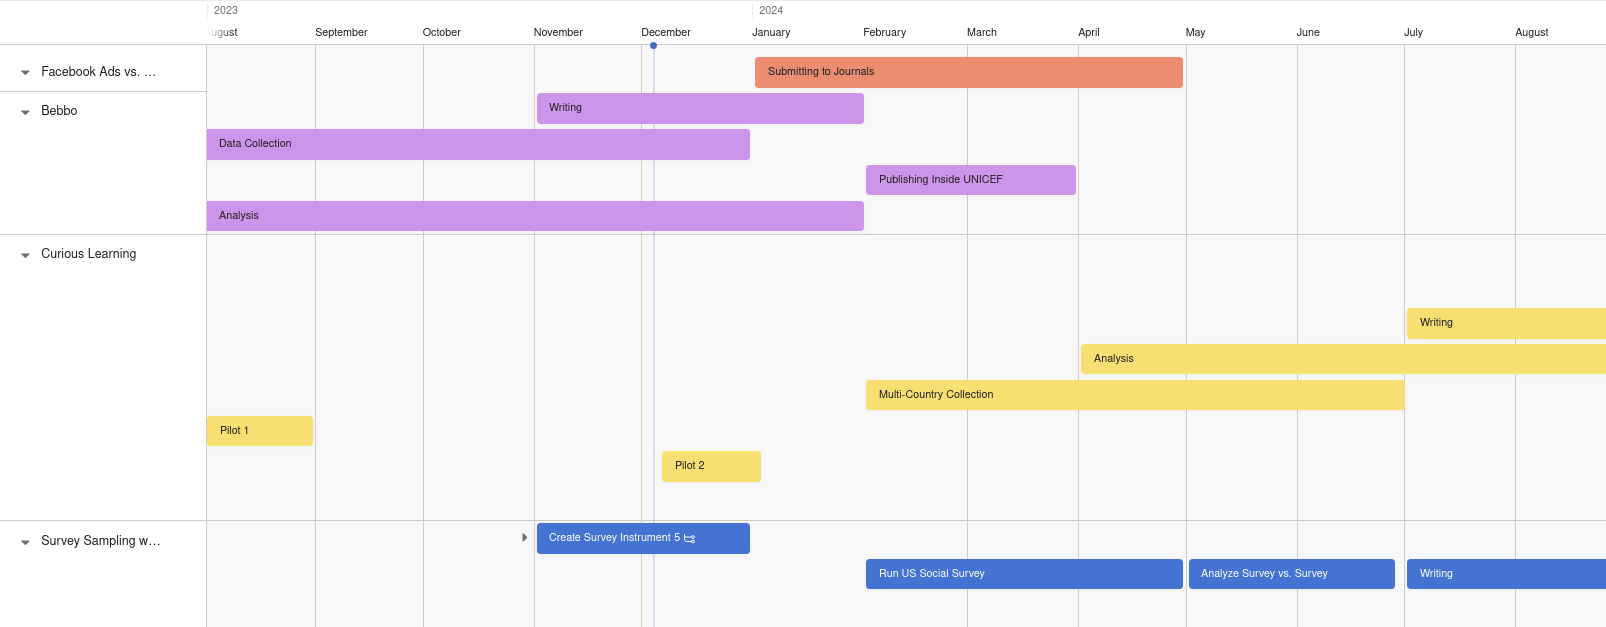
\includegraphics[width=400px]{resources/timeline-2024.png} 
\end{figure}    

\end{frame}


\begin{frame}
  \frametitle{Timeline: 2024-205}

\begin{figure}[]
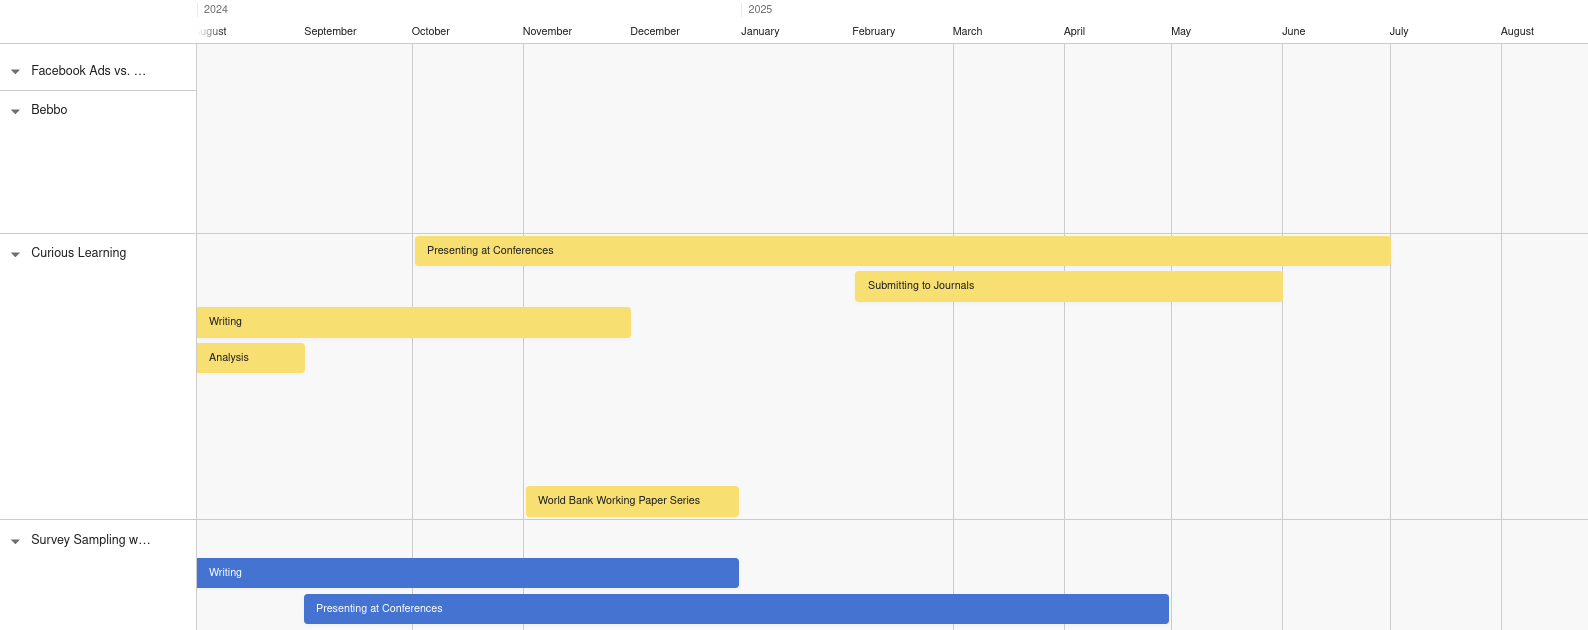
\includegraphics[width=400px]{resources/timeline-2025.png} 
\end{figure}    

\end{frame}


\end{document}

%------------------------------------------------
